\section{Las leyes del movimiento}
  \subsection{Concepto de fuerza}
    \PN Clasificación de un fuerza según contacto:
    \begin{itemize}
      \item \textbf{Fuerza de contacto:} implican contacto físico entre dos objetos.
        \begin{figure}[H]
          \centering
          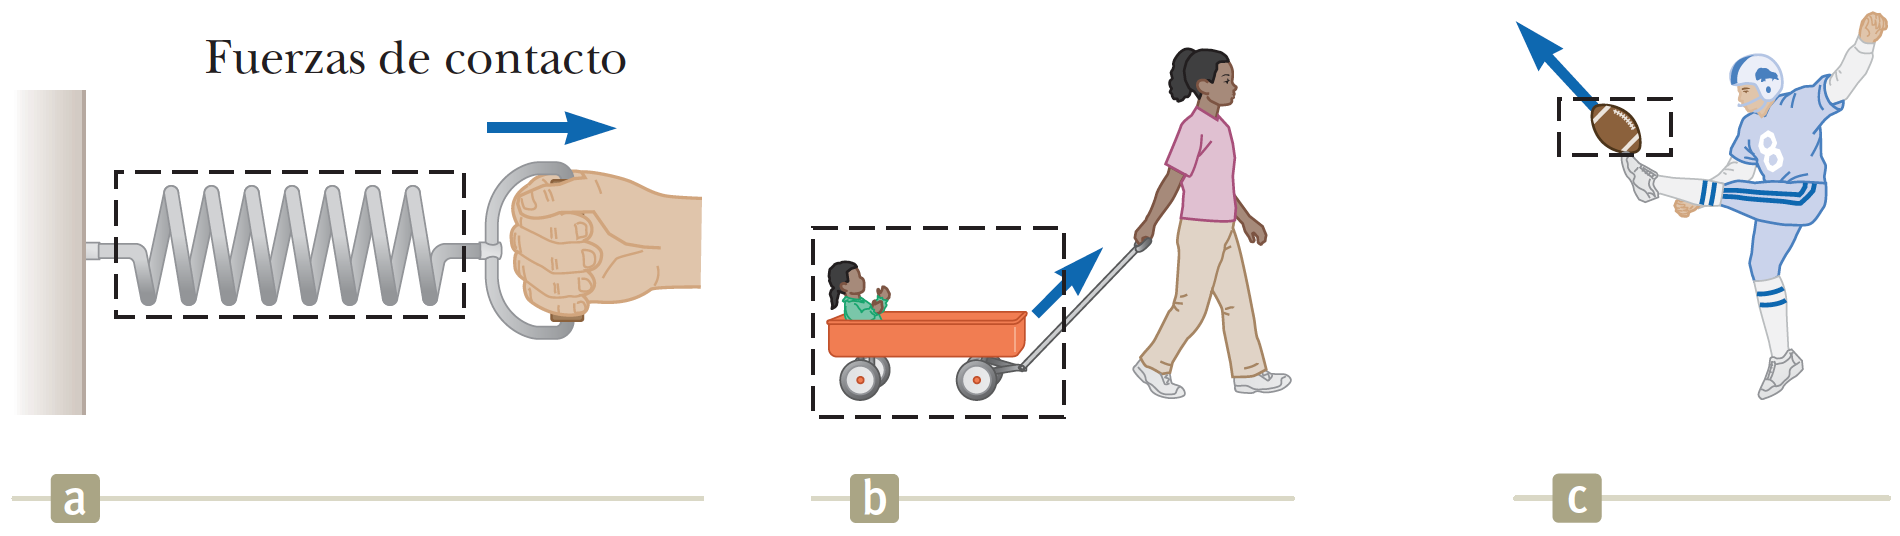
\includegraphics[scale=0.4]{1/graphics_5/figure_0}
          \caption{Una partícula que se mueve en el plano xy se ubica con el vector de posición $\BV{r}$, que se dibuja
          desde el origen hasta la partícula.}
        \end{figure}

      \item \textbf{Fuerza de campo:} no involucran contacto físico entre dos objetos.
        \begin{figure}[H]
          \centering
          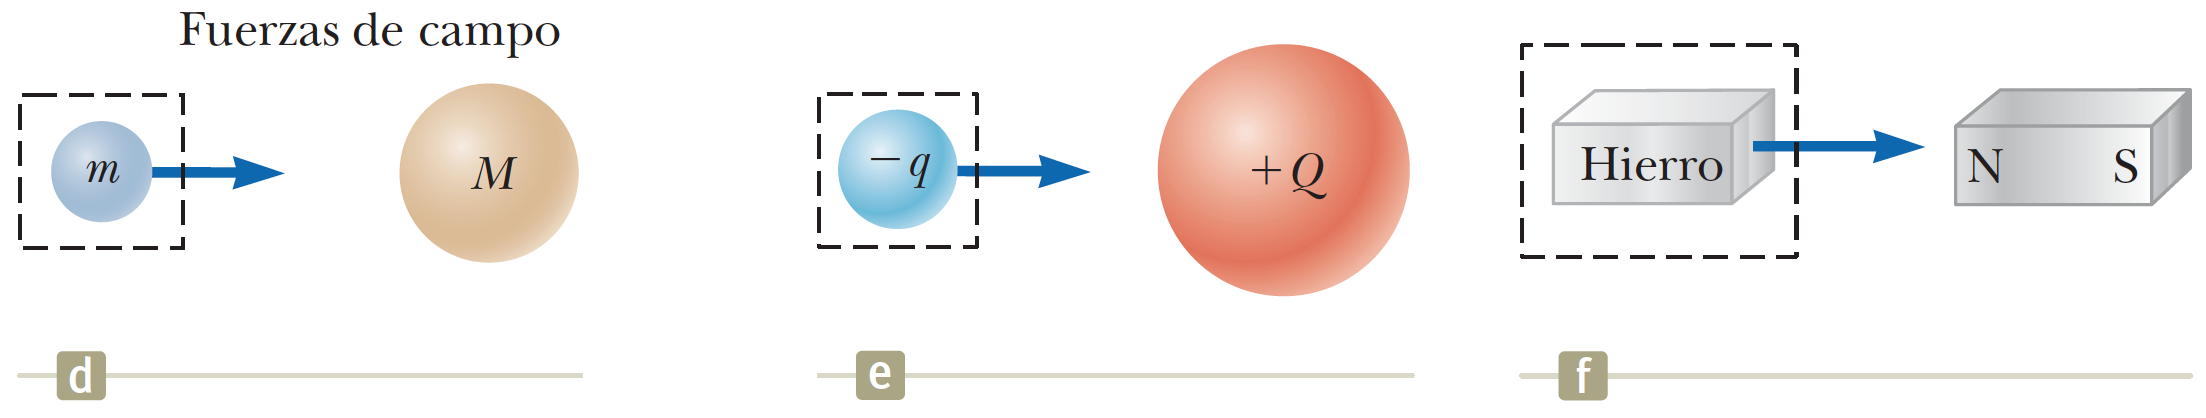
\includegraphics[scale=0.4]{1/graphics_5/figure_1}
          \caption{Una partícula que se mueve en el plano xy se ubica con el vector de posición $\BV{r}$, que se dibuja
          desde el origen hasta la partícula.}
        \end{figure}
    \end{itemize}

    \PN La distinción entre \textit{fuerzas de contacto} y \textit{fuerzas de campo} no es tan clara como se podría
    pensar. Cuando se examinan a nivel atómico, todas las fuerzas que se clasifican como fuerzas de contacto resultan
    ser causadas por fuerzas (de campo) eléctricas. Las únicas \textbf{fuerzas fundamentales} conocidas en la naturaleza
    son todas fuerzas de campo:
    \begin{enumerate}
      \item fuerzas gravitacionales entre objetos
      \item fuerzas electromagnéticas entre cargas eléctricas
      \item fuerzas fuertes entre partículas subatómicas
      \item fuerzas débiles que surgen en ciertos procesos de decaimiento radiactivo
    \end{enumerate}

    \PN En la física clásica sólo interesan las fuerzas gravitacional y electromagnética.

  \subsection{Primera ley de Newton y marcos inerciales}
    \PN La primera ley del movimiento de Newton, a veces llamada \textit{ley de la inercia}, define un conjunto especial
    de marcos de referencia llamados marcos inerciales. Esta ley se puede establecer del modo siguiente:

    \begin{tcolorbox}
      Si un objeto no interactúa con otros objetos, es posible identificar un marco de referencia inercial en el que el
      objeto tiene aceleración cero.
    \end{tcolorbox}

    \PN Tal marco de referencia se llama \textbf{marco de referencia inercial}.

    \PN Se puede plantear un enunciado más práctico de la primera ley del movimiento de Newton:

    \begin{tcolorbox}
      En ausencia de fuerzas externas, y cuando se ve desde un marco de referencia inercial, un objeto en reposo se
      mantiene en reposo y un objeto en movimiento continúa en movimiento con una velocidad constante (esto es, con una
      rapidez constante en una línea recta).
    \end{tcolorbox}

    \PN En otras palabras, cuando ninguna fuerza actúa sobre un objeto, la aceleración del objeto es cero. La tendencia
    de un objeto a resistir cualquier intento por cambiar su velocidad se llama inercia. Se puede concluir que un objeto
    que acelera debe experimentar una fuerza. A su vez, de la primera ley, se puede definir fuerza como aquello que
    causa un cambio en el movimiento de un objeto.

  \subsection{Masa}
    \PN La masa es la propiedad de un objeto que especifica cuánta resistencia muestra un objeto para cambiar su
    velocidad. Los experimentos muestran que mientras más grande sea la masa de un objeto, menos acelera el objeto bajo
    la acción de una fuerza aplicada conocida.

    \PN Suponga que una fuerza que actúa sobre un objeto de masa $m_{1}$ produce un cambio en el movimiento de éste que
    puede cuantificarse mediante la aceleración $\BV{a}_{1}$ del objeto, y la misma fuerza sobre un cuerpo de masa
    $m_{2}$ produce una aceleración $\BV{a}_{2}$. La razón de las dos masas se define como la razón inversa de las
    magnitudes de las aceleraciones producidas por la fuerza:

    \[
      \frac{m_{1}}{m_{2}} \equiv \frac{a_{2}}{a_{1}}
    \]

    \PN La magnitud de la aceleración de un objeto es inversamente proporcional a su masa cuando sobre él actúa una
    fuerza conocida.

    \PN La masa no se debe confundir con el peso. La masa y el peso son dos cantidades diferentes. El peso de un objeto
    es igual a la magnitud de la fuerza gravitacional ejercida sobre el objeto y varía con la posición.

  \subsection{Segunda ley de Newton}
    \PN La segunda ley de Newton responde la pregunta de qué le ocurre a un objeto que tiene una o más fuerzas que
    actúan sobre él. La aceleración de un objeto es directamente proporcional a la fuerza que actúa sobre él:
    $\BV{F} \propto \BV{a}$. La magnitud de la aceleración de un objeto es inversamente proporcional a su masa,
    $\abs{\BV{a}} \propto \frac{1}{m}$.

    \PN Estas observaciones experimentales se resumen en la segunda ley de Newton:

    \begin{tcolorbox}
      Cuando se ve desde un marco de referencia inercial, la aceleración de un objeto es directamente proporcional a la
      fuerza neta que actúa sobre él e inversamente proporcional a su masa:

      \[
        \BV{a} \propto \frac{\sum \BV{F}}{m}
      \]
    \end{tcolorbox}

    \PN Si se elige una constante de proporcionalidad 1, se relaciona masa, aceleración y fuerza a través del siguiente
    enunciado matemático de la segunda ley de Newton:

    \[
      \sum \BV{F} = m \BV{a}
    \]

    \PN La fuerza neta sobre un objeto es la suma vectorial de todas las fuerzas que actúan sobre el objeto. A veces a
    la fuerza neta se le referirá como fuerza total, fuerza resultante o fuerza desbalanceada.

  \subsection{Fuerza gravitacional y peso}
    \PN La fuerza de atracción que ejerce la Tierra sobre un objeto se llama \textbf{fuerza gravitacional} $\BV{f}_{g}$.
    Esta fuerza se dirige hacia el centro de la Tierra y su magnitud se llama peso del objeto. Al aplicar la segunda ley
    de Newton $\sum \BV{F} = m \BV{a}$ a un objeto en caída libre de masa $m$, con $\BV{a} = \BV{g}$ y
    $\sum \BV{F} = \BV{F}_{g}$ se obtiene:

    \[
      \BV{F}_{g} = m \BV{g}
    \]

    \PN Por lo tanto, el peso de un objeto, al definirse como la magnitud de $\BV{F}_{g}$, está dado por:

    \[
      F_{g} = m g
    \]

    \PN Esta ecuación cuantifica la fuerza gravitacional sobre el objeto, pero note que no requiere que el objeto se
    mueva. Incluso para un objeto fijo o para un objeto sobre el que actúan varias fuerzas, la ecuación se puede aplicar
    para calcular la magnitud de la fuerza gravitacional. La masa $m$ en la ecuación anterior establece la intensidad de
    la atracción gravitacional entre el objeto y la Tierra. Este papel es por completo diferente del descrito antes para
    la masa: medir la resistencia al cambio en movimiento como respuesta a una fuerza externa. En ese papel, la masa
    también es llamada \textbf{masa inercial}. Por ende, la $m$ en la ecuación anterior se llama
    \textbf{masa gravitacional}.

  \subsection{Tercera ley de Newton}
    \PN Las fuerzas son \textit{interacciones} entre dos objetos, este importante principio se conoce como
    \textbf{tercera ley de Newton}.

    \begin{tcolorbox}
      Si dos objetos interactúan, la fuerza $\BV{F}_{12}$ que ejerce el objeto 1 sobre el objeto 2 es igual en magnitud
      y opuesta en dirección a la fuerza $\BV{F}_{21}$ que ejerce el objeto 2 sobre el objeto 1:

      \[
        \BV{F}_{12} = - \BV{F}_{21}
      \]
    \end{tcolorbox}

    \PN Cuando sea importante designar fuerzas como interacciones entre dos objetos, se usará esta notación de
    subíndices, donde $\BV{F}_{ab}$ significa \textquotedblleft la fuerza ejercida por a sobre b\textquotedblright.

    \vspace{3mm}
    \PN La tercera ley se ilustra en la siguiente figura. La fuerza que el objeto 1 ejerce sobre el objeto 2 se llama
    popularmente \textit{fuerza de acción}, y la fuerza del objeto 2 sobre el objeto 1 se llama
    \textit{fuerza de reacción}.

    \begin{figure}[H]
      \centering
      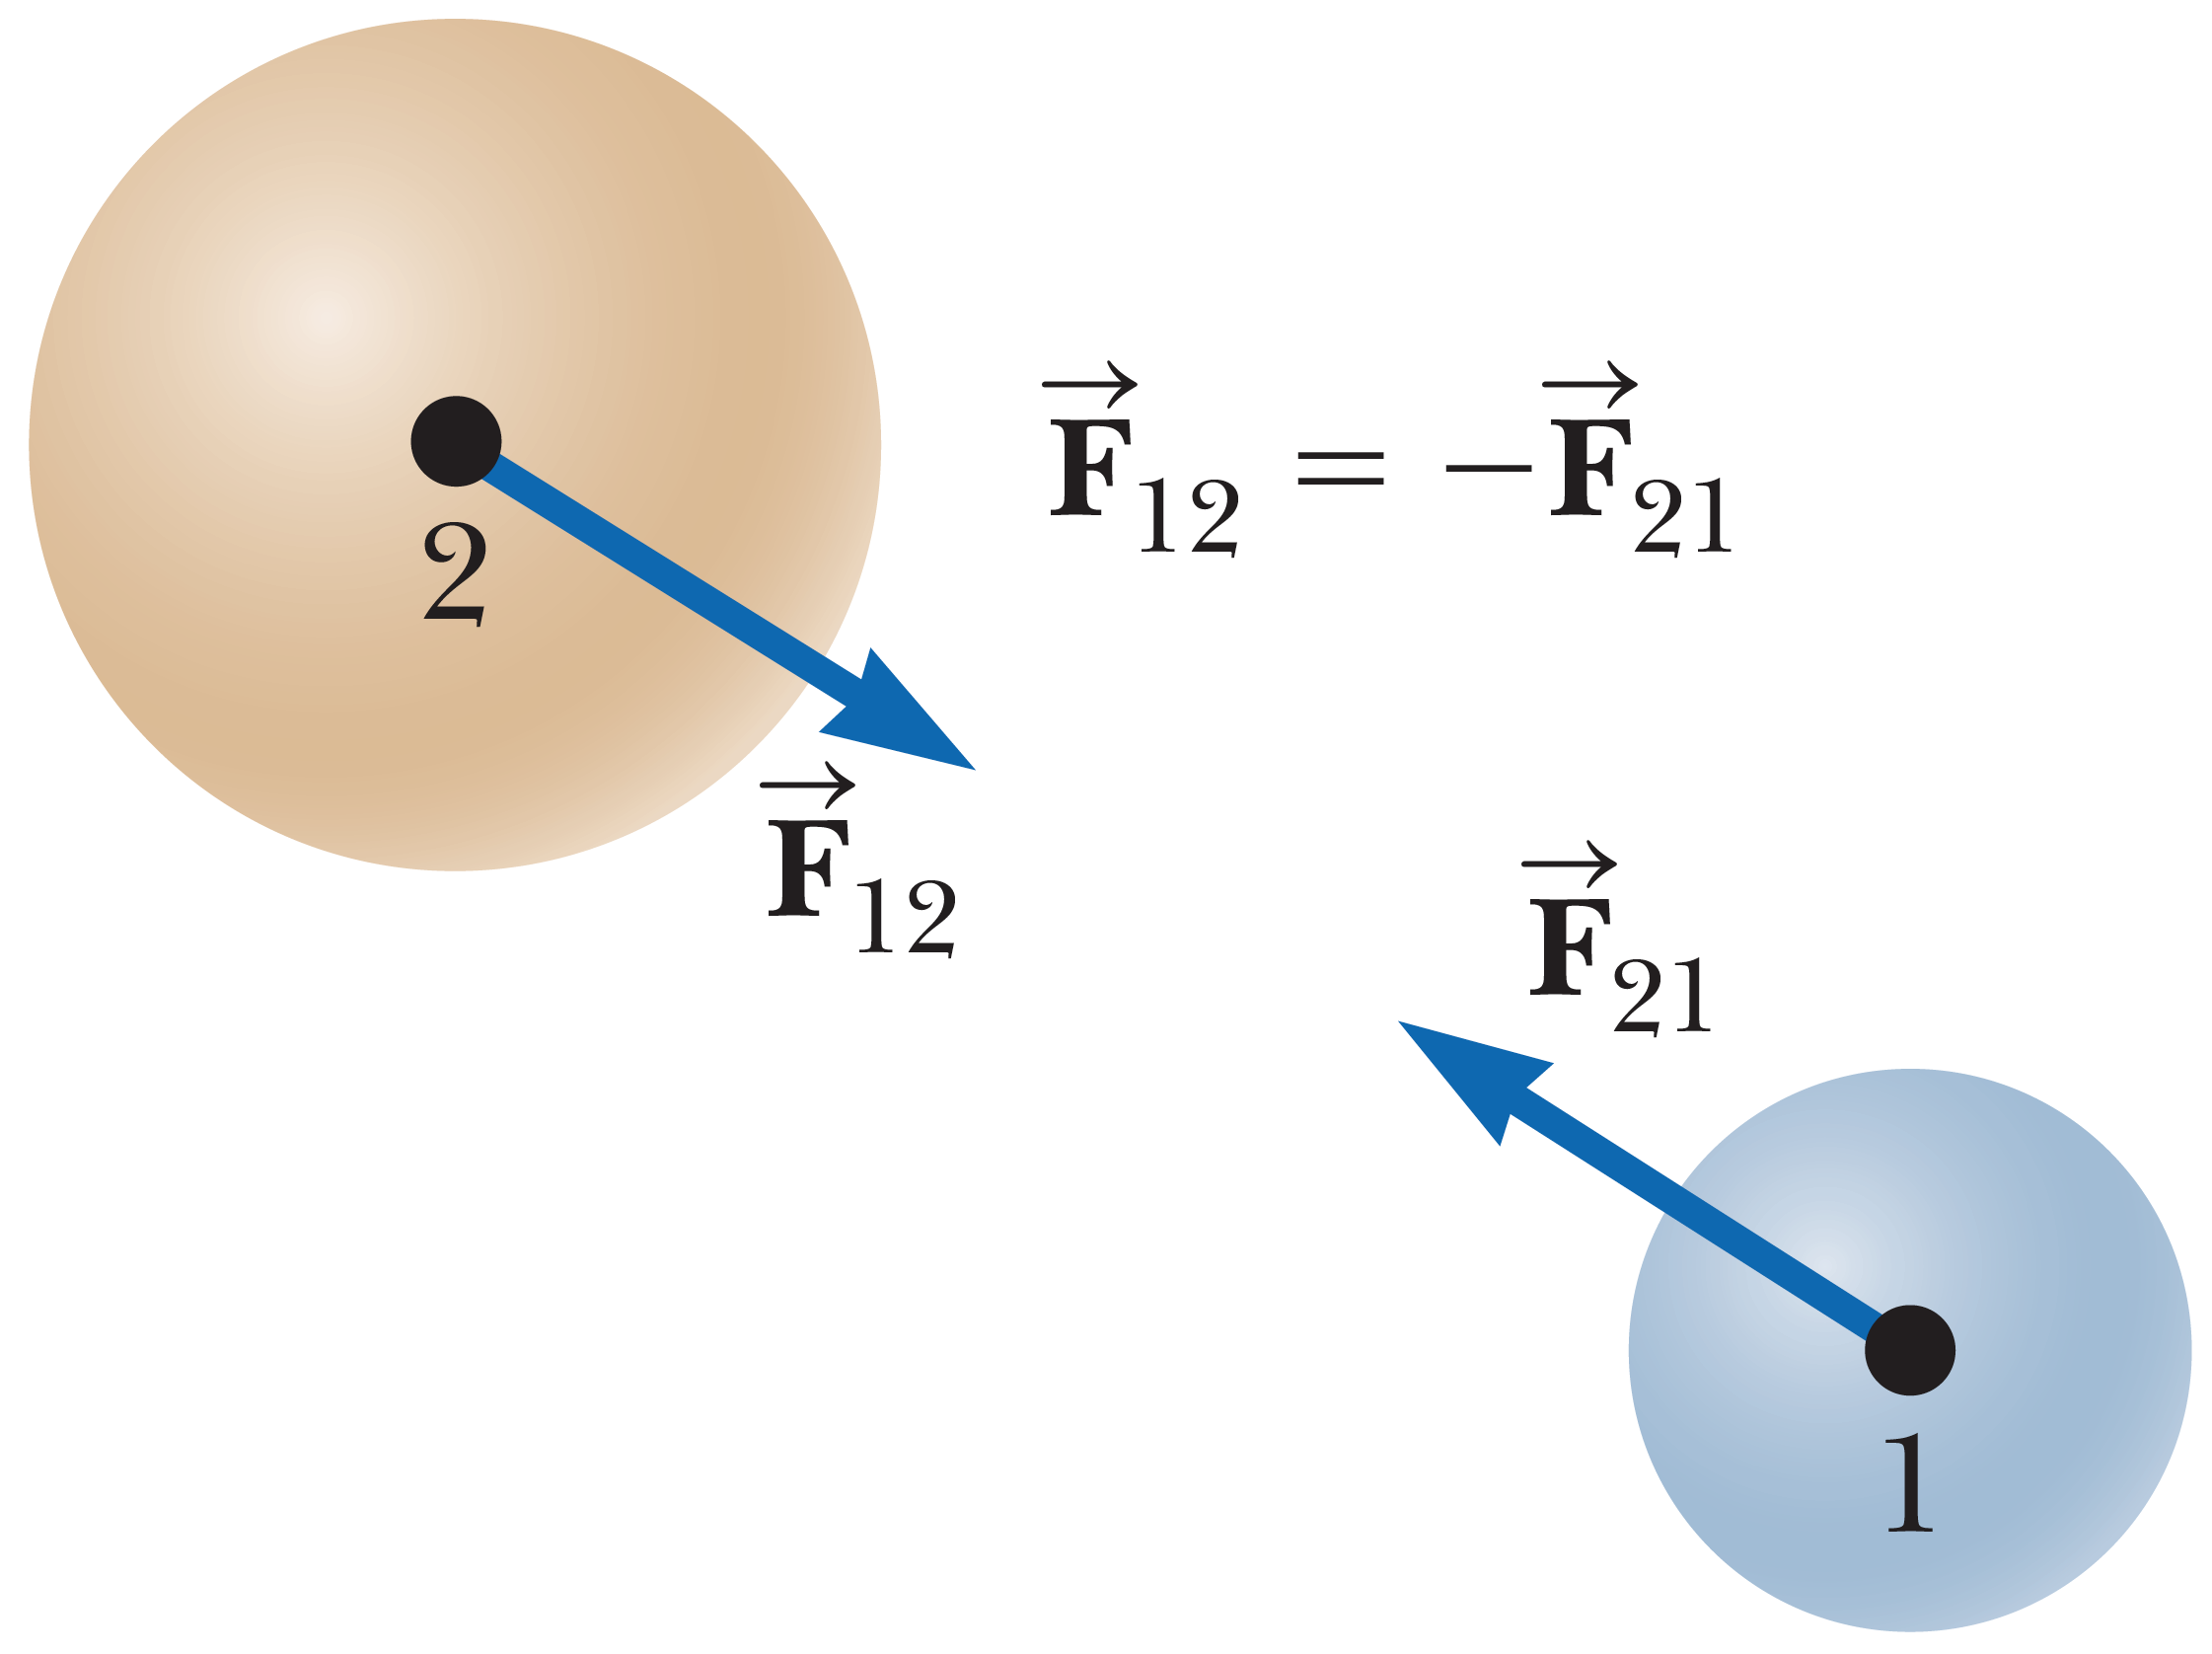
\includegraphics[scale=0.15]{1/graphics_5/figure_2}
      \caption{Tercera ley de Newton. La fuerza $\BV{F}_{12}$ que ejerce el objeto 1 sobre el objeto 2 es igual en
      magnitud y opuesta en dirección a la fuerza $\BV{F}_{21}$ que ejerce el objeto 2 sobre el objeto 1.}
    \end{figure}

    \PN Considere un monitor de computadora en reposo sobre una mesa, como en la figura siguiente. El monitor no acelera
    porque lo sostiene la mesa (t). La mesa ejerce sobre el monitor una fuerza hacia arriba $\BV{n} = \BV{F}_{tm}$,
    llamada \textbf{fuerza normal}. En general, siempre que un objeto esté en contacto con una superficie, ésta ejerce
    una fuerza normal sobre el objeto. Puesto que el monitor tiene aceleración cero, la segunda ley de Newton aplicada
    al monitor produce $\sum \BV{F} = \BV{n} + m \BV{g} = 0$, de modo que $n = mg$. La fuerza normal equilibra la fuerza
    gravitacional sobre el monitor, de modo que la fuerza neta sobre el monitor es cero.

    \begin{figure}[H]
      \centering
      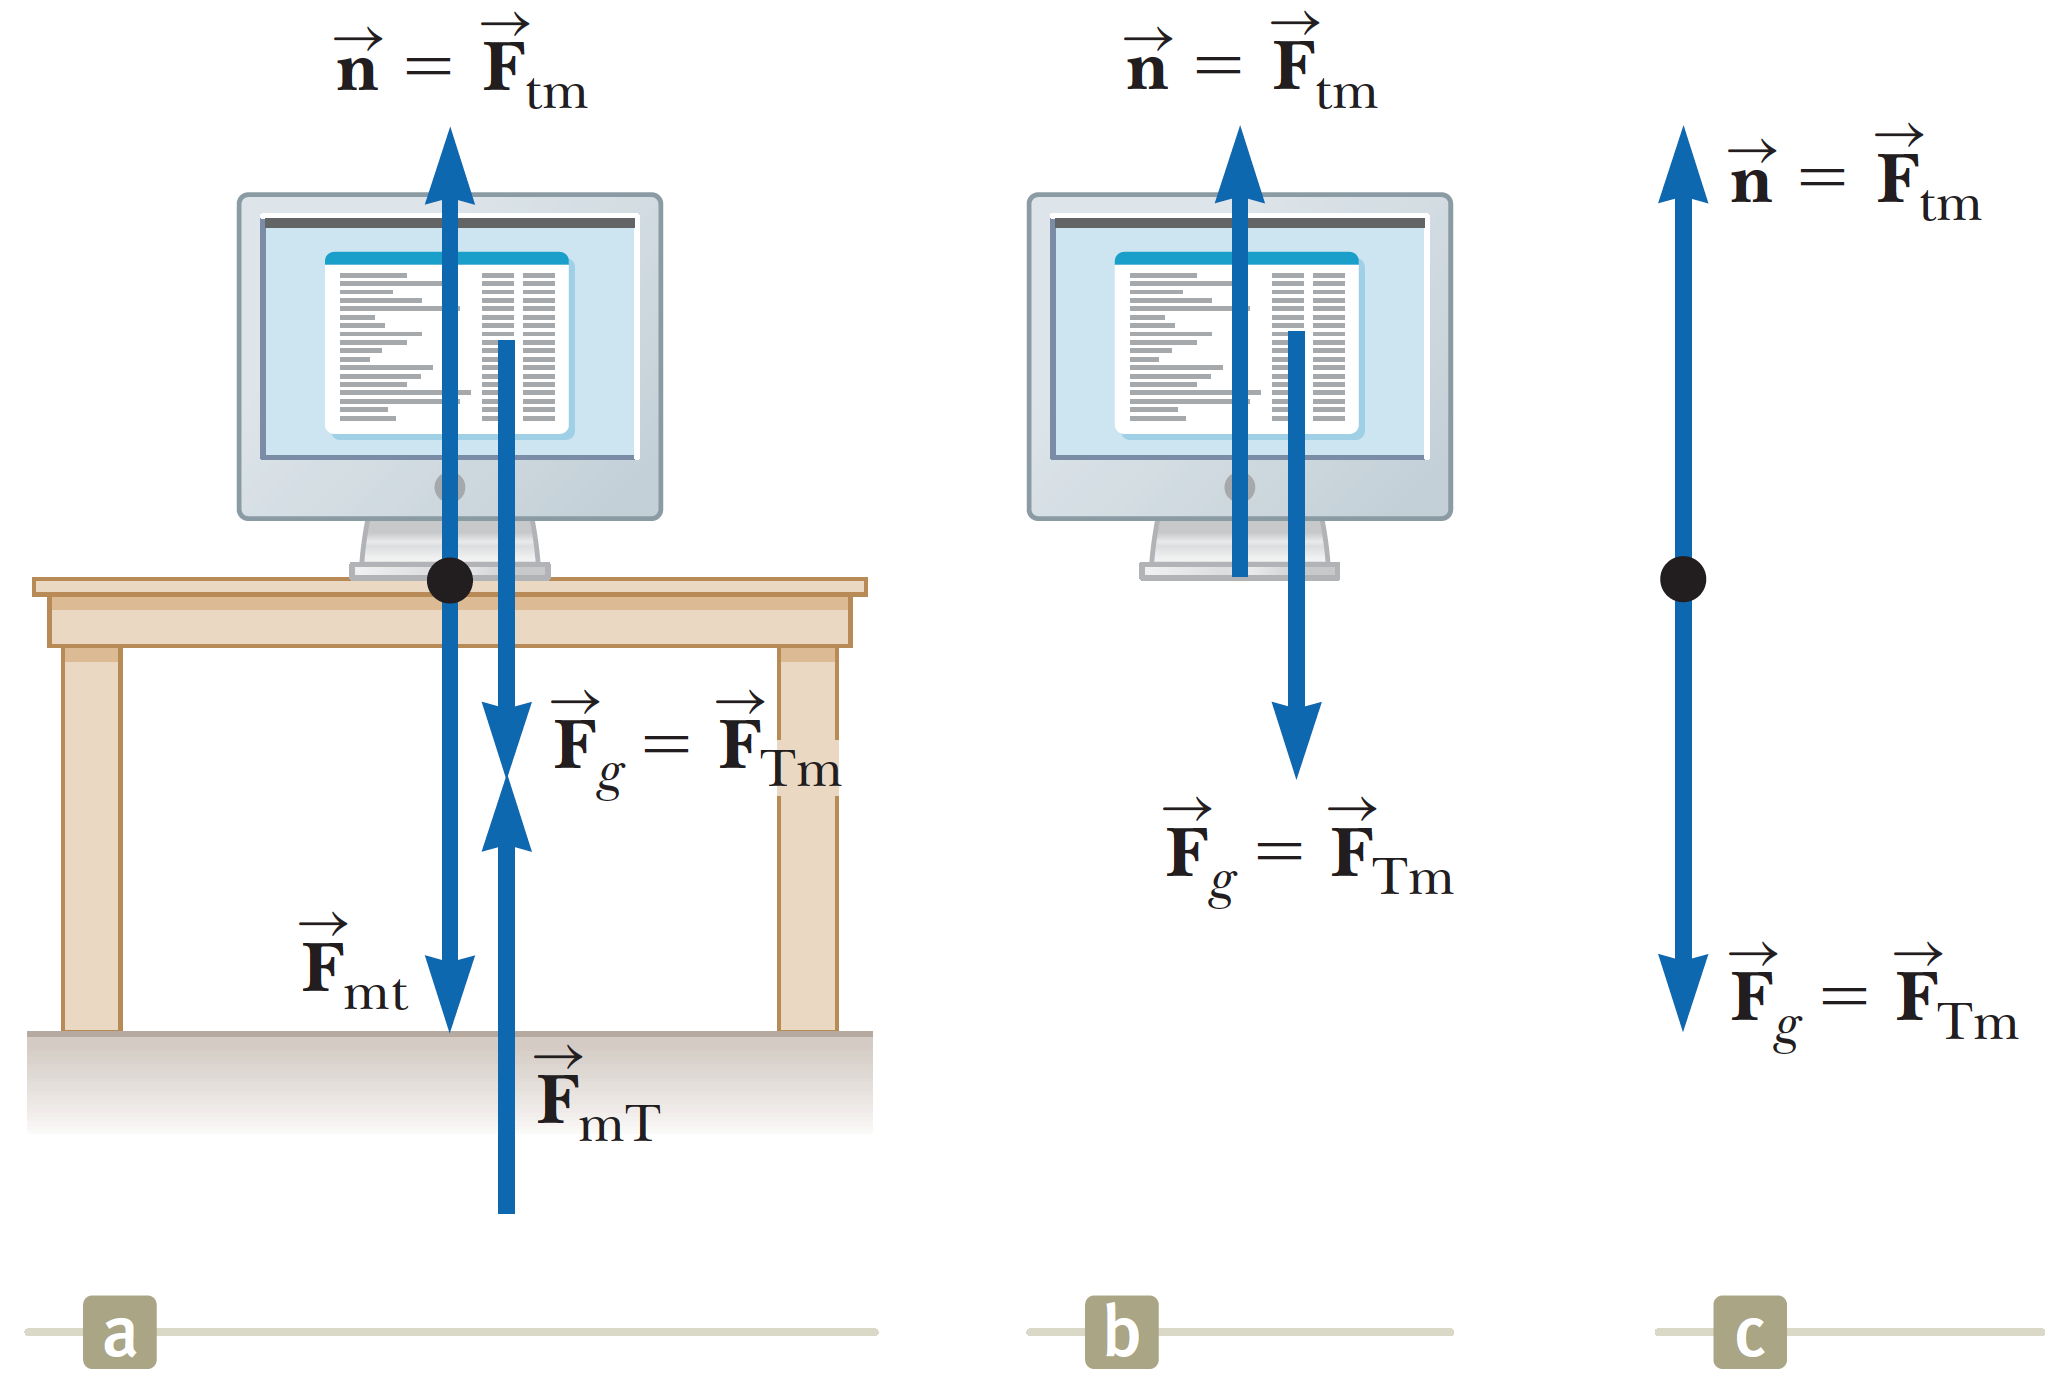
\includegraphics[scale=0.3]{1/graphics_5/figure_3}
      \caption{(a) Cuando un monitor de computadora está en reposo sobre una mesa, las fuerzas que actúan sobre el
      monitor son la fuerza normal $\BV{n}$ y la fuerza gravitacional $\BV{F}_{g}$. La reacción a $\BV{n}$ es la fuerza
      $\BV{F}_{mt}$ que ejerce el monitor sobre la mesa. La reacción a $\BV{F}_{g}$ es la fuerza $\BV{F}_{mT}$ que
      ejerce el monitor sobre la Tierra. (b) Un diagrama de fuerzas muestra las fuerzas sobre el monitor. (c) Un
      diagrama de cuerpo libre mostrando al monitor como un punto negro con las fuerzas actuando sobre él.}
    \end{figure}

  \subsection{Análisis de modelos utilizando la segunda ley de Newton}
    \PN En esta sección se discuten dos análisis de modelos para resolver problemas en que los objetos están en
    equilibrio $(\BV{a} = 0)$ aceleran a lo largo de una línea recta bajo la acción de fuerzas externas constantes. Se
    desprecian los efectos de la fricción en aquellos problemas que involucran movimiento, que es equivalente a afirmar
    que la superficie \textit{no tiene fricción}. Por lo general, se ignora la masa de cualquier soga, cuerda o cable
    involucrado.

    \PN Cuando una cuerda unida a un objeto está jalando al objeto, la cuerda ejerce una fuerza sobre el objeto en una
    dirección que se aleja del objeto, paralela a la cuerda. La magnitud T de dicha fuerza se llama tensión en la cuerda.

    \subsubsection{Análisis de modelo: partícula en equilibrio}
      \PN Si la aceleración de un objeto representado como partícula es cero, el objeto se considera con el modelo de
      \textbf{partícula en equilibrio}. En este modelo, la fuerza neta sobre el objeto es cero:

      \[
        \sum \BV{F} = 0
      \]

    \subsubsection{Análisis de modelo: partícula bajo una fuerza neta}
      \PN Si un objeto experimenta una aceleración, su movimiento se puede analizar con el modelo de partícula bajo una
      fuerza neta. La ecuación apropiada para este modelo es la segunda ley de Newton:

      \[
        \sum \BV{F} = m \BV{a}
      \]

  \subsection{Fuerzas de fricción}
    \PN Cuando un objeto está en movimiento, ya sea sobre una superficie o en un medio viscoso como aire o agua, existe
    resistencia al movimiento porque el objeto interactúa con su entorno. A tal resistencia se le llama fuerza de
    fricción. Las fuerzas de fricción son muy importantes en la vida cotidiana. Permiten que uno camine o corra y son
    necesarias para el movimiento de los vehículos con ruedas.

    \begin{figure}[H]
      \minipage{0.45\textwidth}
      \centering
      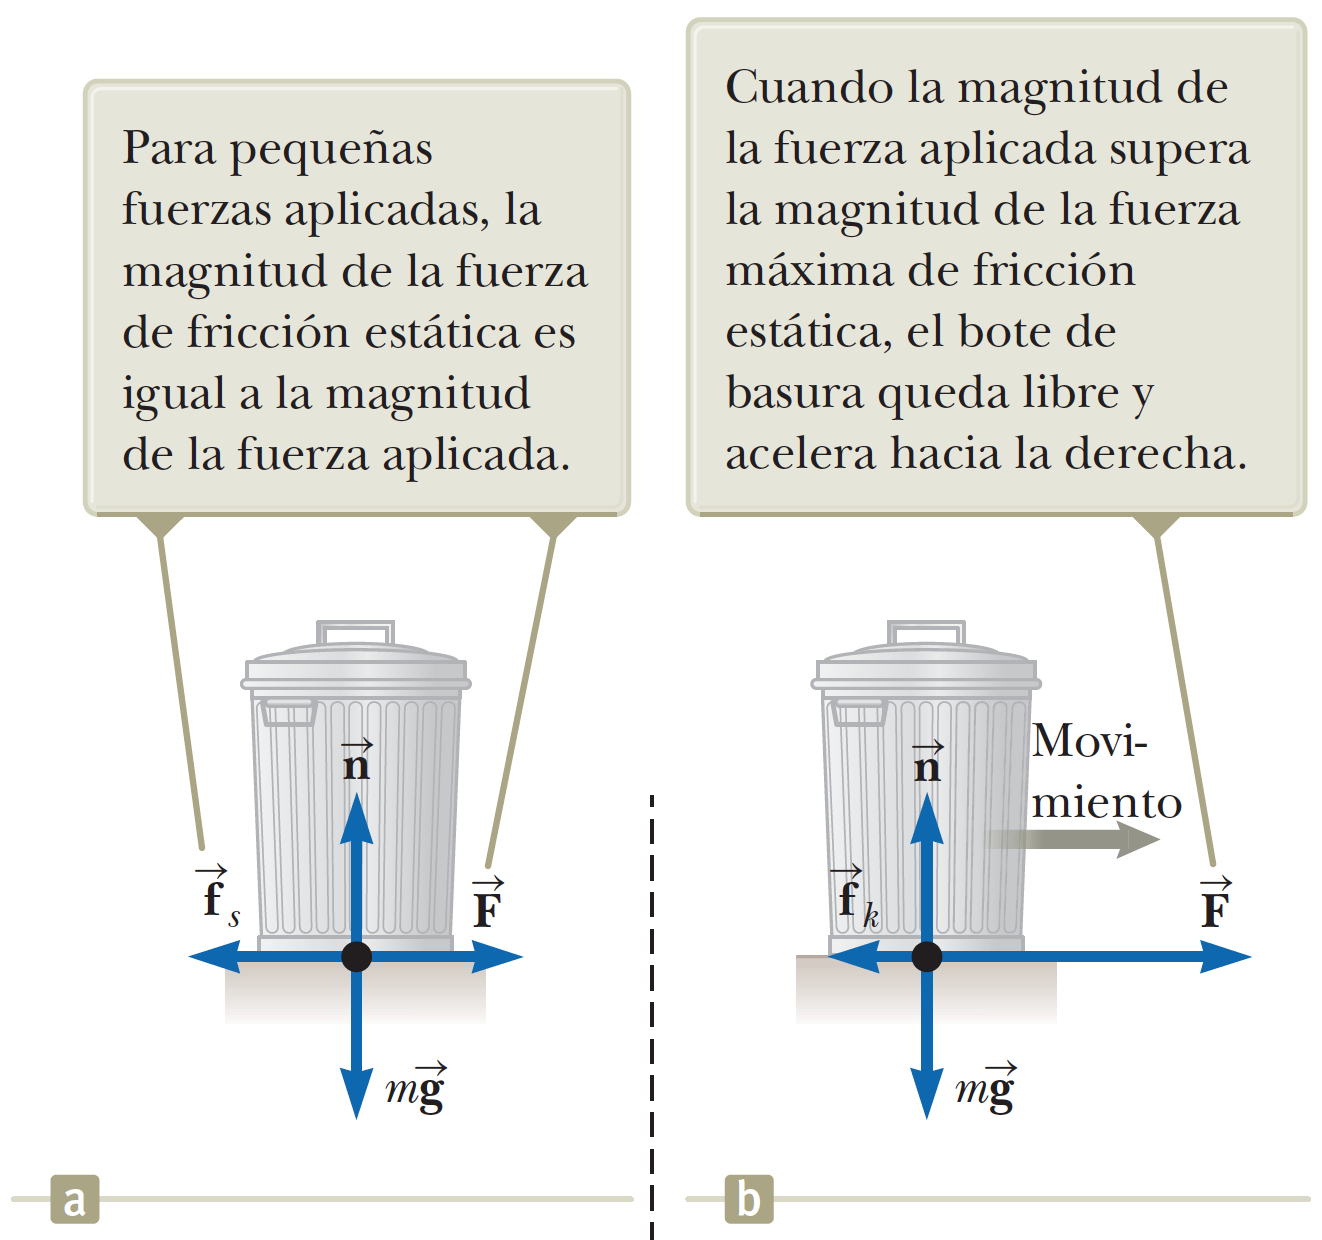
\includegraphics[scale=0.3]{1/graphics_5/figure_4a}
      \caption{Cuando jala un bote de basura, la dirección de la fuerza de fricción $\BV{f}$ entre el bote y una
      superficie rugosa es opuesta a la dirección de la fuerza aplicada $\BV{F}$.}
      \endminipage\hspace{8mm}
      \minipage{0.45\textwidth}
      \centering
      \vspace{18mm}
      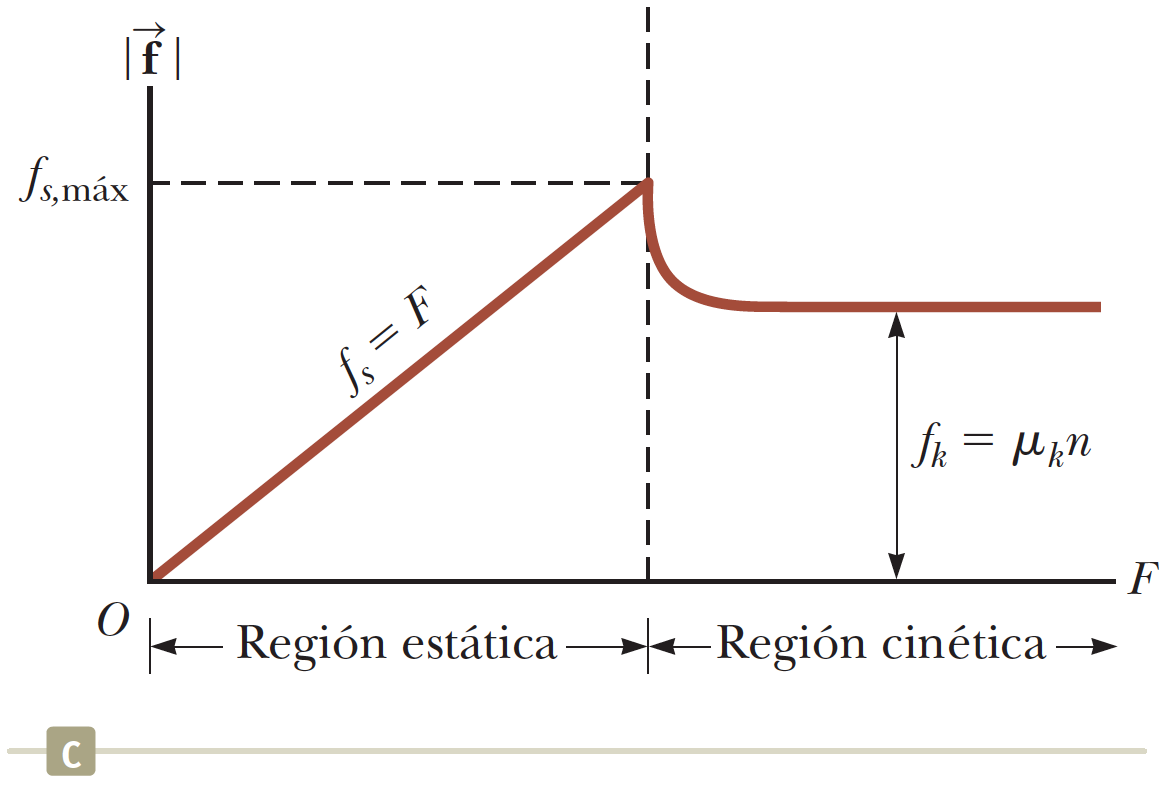
\includegraphics[scale=0.3]{1/graphics_5/figure_4b}
      \caption{Gráfica de fuerza de fricción en función de la fuerza aplicada. Note que $f_{s,max} \geq f_{k}$.}
      \endminipage
    \end{figure}

    \PN A la fuerza de fricción para un objeto en movimiento se le llama \textbf{fuerza de fricción cinética}
    $\BV{f}_{k}$. La fuerza neta $F-f_{k}$ en la dirección $x$ produce una aceleración hacia la derecha, de acuerdo con
    la segunda ley de Newton. Si $F = f_{k}$, la aceleración es cero y el bote de basura se mueve hacia la derecha con
    rapidez constante. Si la fuerza aplicada $\BV{F}$ se elimina del bote en movimiento, la fuerza de fricción
    $\BV{f}_{k}$ que actúa hacia la izquierda proporciona una aceleración del bote de basura en la dirección $-x$ y al
    final lo lleva al reposo.

    \PN Las siguientes descripciones de la fuerza de fricción están en función de las observaciones experimentales y
    sirven como el modelo que se usará para fuerzas de fricción en resolución de problemas:

    \begin{itemize}
      \item La magnitud de la fuerza de fricción estática entre cualesquiera dos superficies en contacto puede tener los
      valores:
        \[
          f_{s} \geq \mu_{s} n
        \]

      \PN donde la constante adimensional $\mu_{s}$ se llama \textbf{coeficiente de fricción estática} y $n$ es la
      magnitud de la fuerza normal que ejerce una superficie sobre la otra. La igualdad se cumple cuando las superficies
      están a punto de deslizarse, esto es, cuando $f_{s} = f_{s, max} = \mu_{s} n$. Esta situación se llama
      \textbf{movimiento inminente}.

      \item La magnitud de la fuerza de fricción cinética que actúa entre dos superficies es:
        \[
          f_{k} = \mu_{k} n
        \]

        \PN donde $\mu_{k}$ se llama \textbf{coeficiente de fricción cinética}. Aunque el coeficiente de fricción
        cinética varía con la rapidez, por lo general en este texto se despreciará cualquiera de tales variaciones.

      \item Los valores de $\mu_{k}, \mu_{s}$ dependen de la naturaleza de las superficies, pero $\mu_{k}$ por lo
      general es menor que $\mu_{s}$.

      \item La dirección de la fuerza de fricción sobre un objeto es paralela a la superficie con la que el objeto está
      en contacto y opuesta al movimiento real (fricción cinética) o al movimiento inminente (fricción estática) del
      objeto en relación con la superficie.

      \item Los coeficientes de fricción son casi independientes del área de contacto entre las superficies.
    \end{itemize}
